\subsection{Daten plotten}
\label{sec:potdata}
Das Module \textsf{Basemap} bietet die Möglichkeit die Plotroutinen von \textsf{pyplot} zu benutzen, da es die Karte mit \textsf{matplotlib} erstellt. Die Karte ist im Grunde ein \textsf{AxesImage}, auf dem dann die entsprechenden Operationen ausgeführt werden. Daher kann man auch die Plotroutinen von \textsf{pyplot} aufrufen da diese ebenfalls mit \textsf{AxesImages} arbeiten. Wenn man mit \textsf{pyplot} zeichnet muss man beachten, dass die Koordinaten, die man angeben muss, in den Projektionskoordinaten der Karte anzugeben sind. Dabei ist die \textsf{Basemap} Klasse sehr hilfreich, sie rechnet nämlich Koordinaten in Längen- und Breitengrad in die Projektionskoordinaten um. Dazu mus man einfach die \textsf{basemap} Instanz mit den Koordinaten als Parameter aufrufen. Dabei können auch mehrere Koordinaten übergeben werden, indem man zwei Felder übergibt.\\
\lstinputlisting{/Users/student/seminar/bsp/bspconvert.py}
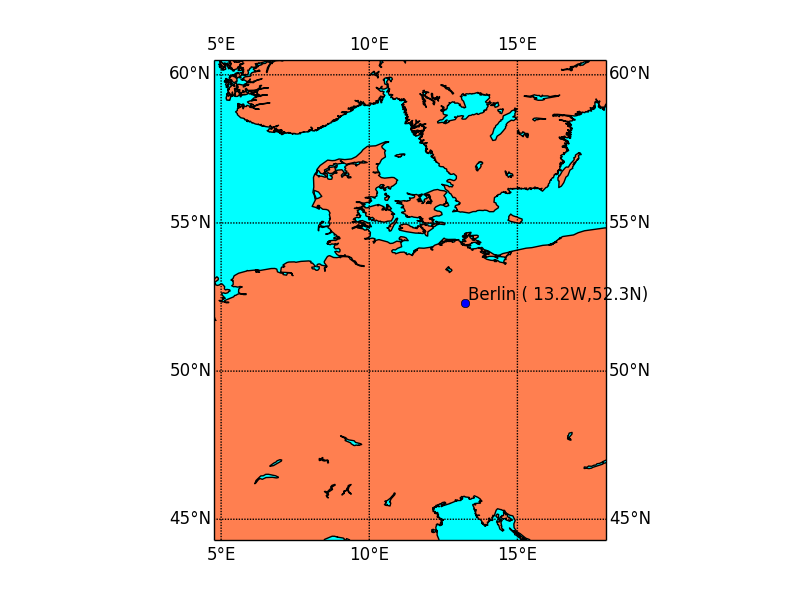
\includegraphics[scale=0.4]{/Users/student/seminar/bsp/bspconvert}\newpage
\subsubsection{Isobaren plotten}
um Isobaren zu plotten braucht man ein zweidimensionales Datenfeld mit den Werten und zwei Felder mit den dazu gehörigen Koordinaten. Diese kann man dann einfach mit Hilfe der Funktion \textsf{contour(x, y, data, *args, **kwargs)} plotten. Die Funktion \textsf{contour} zeichnet Isobarenlinien. Mit der Funktion \textsf{contourf(x, y, data, *args, **kwargs)} werden diese auch gefüllt. Den beiden Funktionen kann man ein \textsf{colormap} Objekt im Parameter \textsf{cmap} übergeben. Dieser Parameter wird dann einfach an \textsf{pyplot} weitergegeben. Darüber kann man den Farbverlauf der Isobaren steuern. Über den Parameter \textsf{levels} kann man angeben welche Wertelevel gezeichnet werden sollen.\\
\lstinputlisting{/Users/student/seminar/bsp/bspcontur.py}
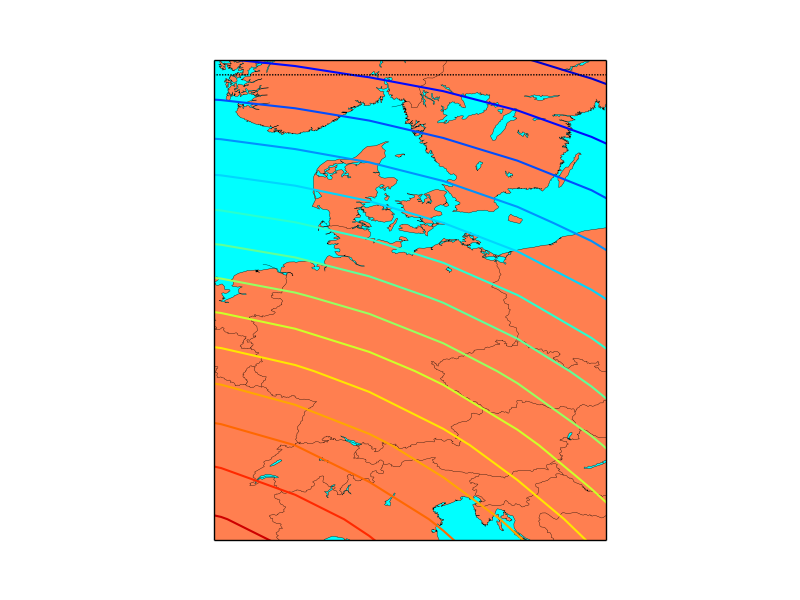
\includegraphics[scale=0.4]{/Users/student/seminar/bsp/bspcont}
Mit der Funktion \textsf{contourf()} muss man aufpassen, dass die Graphik nicht vom Hintergrund übermalt wird. Daher habe ich in dem Beispiel den Kontinent nicht gefüllt.\\
\lstinputlisting{/Users/student/seminar/bsp/bspconturf.py}
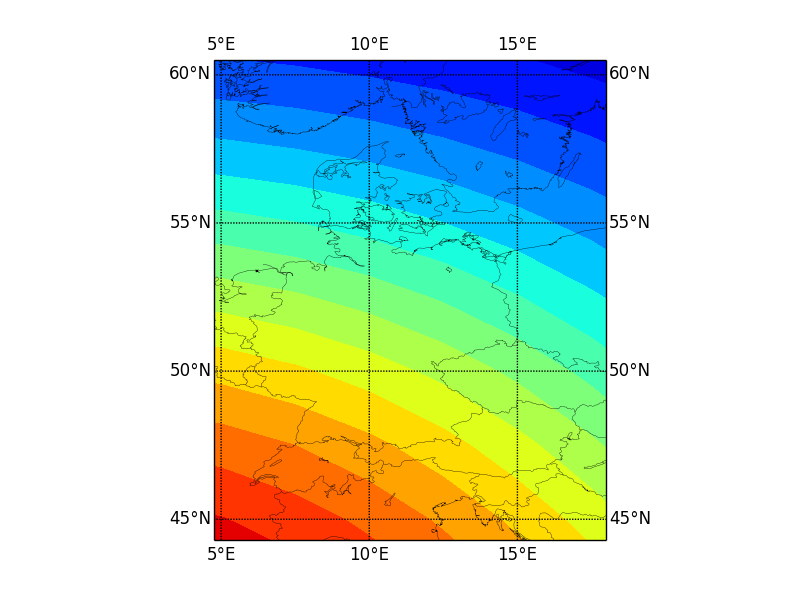
\includegraphics[scale=0.4]{/Users/student/seminar/bsp/bspcontf}\newpage 
\subsubsection{Windmarken plotten}
Mit der Funktion \textsf{barbs(**kw)} kann man einfach Windmarken plotten. Dazu übergibt man der Funktion die Koordinaten der Marke und die Koordinaten des Endpunkts des Vektors der dargestellt werden soll. Die Form der Marke wird durch die Länge des Vektors bestimmt. Eine Flagge bedeutet einen Wert von 50, ein voller Balken 10, ein halber Balken 5. Mit dem Parameter \textsf{barb\_increments} kann man eigene Werte festlegen. Dafür wird dem Parameter ein \textsf{dictionary} mit den \textsf{Schlüsseln} \textsf{half, full, flag} übergeben. Mit dem Parameter \textsf{length} kann man die Länge der Fähnchen in Punkten angeben, der Rest der Marke wird dagegen skaliert.\\
\lstinputlisting{/Users/student/seminar/bsp/bspbarbs.py}
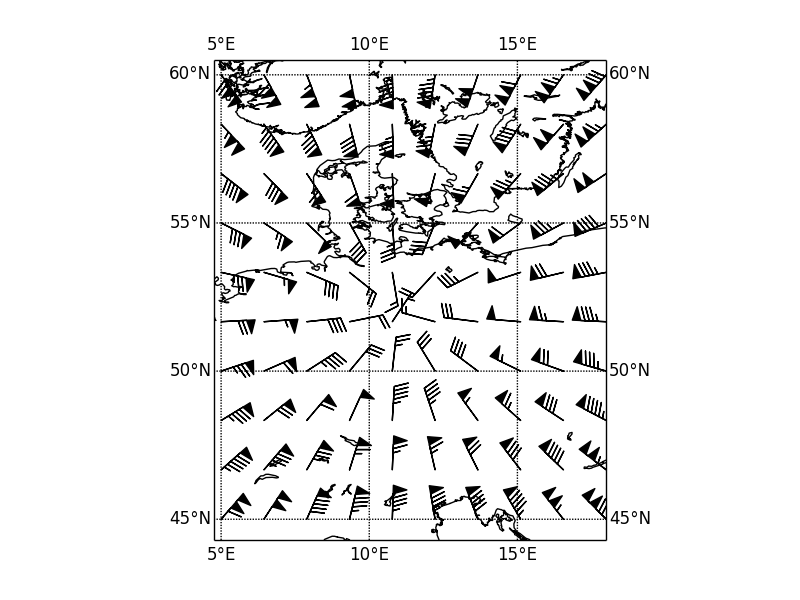
\includegraphics[scale=0.4]{/Users/student/seminar/bsp/bspbarbs}\newpage 
\subsubsection{Windvektoren plotten}
  Mit der Funktion \textsf{quiver(**kw)} kann man Vektoren plotten. Hierbei werden wieder 2 Koordinaten angegeben, wie bei dem Plotten von Windmarken. Mit den Parametern \textsf{u,v} wird ein Vektor übergeben der gezeichnet werden soll. Mit den Parametern \textsf{scale, scale\_units} kann man bestimmen wie lang die Vektoren werden. Je kleiner der \textsf{scale} Parameter desto größer wird der Vektor. Wenn man bei diesen Parametern nichts angibt wird der Wert automatisch aus den zu zeichnenden Vektoren ermittelt.\\
  \lstinputlisting{/Users/student/seminar/bsp/bspquiver.py}
  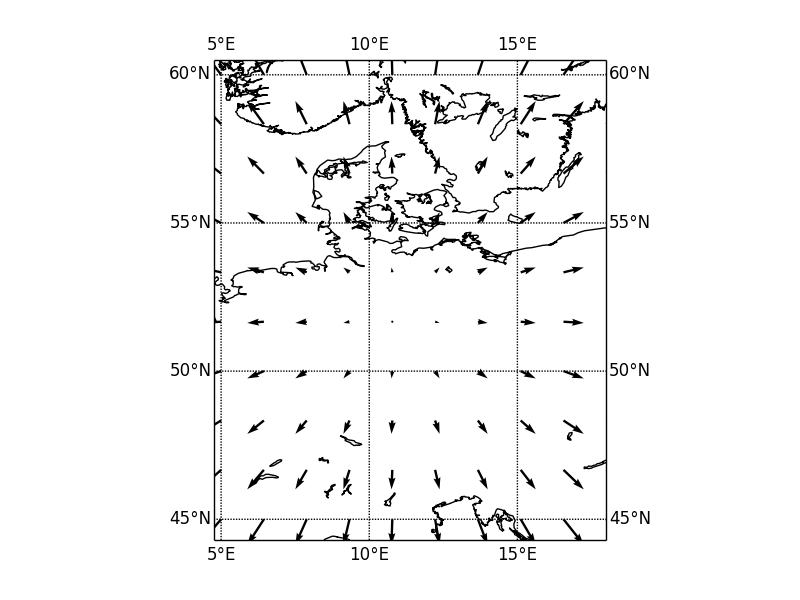
\includegraphics[scale=0.4]{/Users/student/seminar/bsp/bspquiver}\newpage 
  \subsubsection{gekrümmte Strecken plotten}
  Um Strecken wie zum Beispiel eine Flugroute von New York nach London zu plotten, benutzt man am Einfachsten die Funktion \textsf{drawgreatcircle(lon1, lat1, lon2, lat2, del\_s=100.0, **kwargs)}. Diese Funktion zeichnet einen Bogen von den Koordinaten \textsf{lon1,lat1} nach \textsf{lon2,lat2} dabei werden Punkte alle \textsf{del\_s} km ermittelt. Diese Punkte kann man sich auch mit der Funktion \textsf{gcpoints(lon1, lat1, lon2, lat2, points)} berechnen lassen.\\
  \lstinputlisting{/Users/student/seminar/bsp/bspgreatcirc.py}
  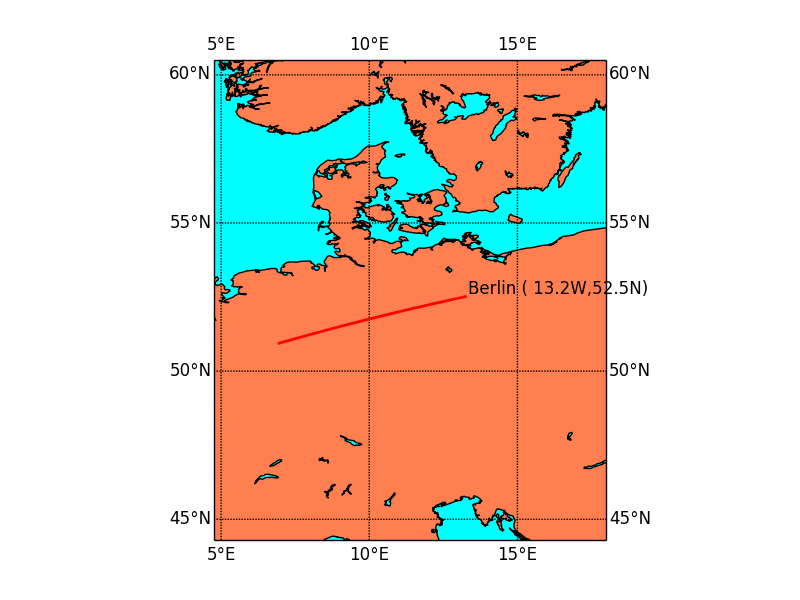
\includegraphics[scale=0.4]{/Users/student/seminar/bsp/bspgreatcirc}\newpage 
  \subsubsection{Viele Punkte plotten}
  Mit der Funktion \textsf{scatter(x, y, s=20, c=u'b', marker=u'o', cmap=None, norm=None, vmin=None, vmax=None, alpha=None, linewidths=None, verts=None, hold=None, **kwargs)} kann man Marken plotten. Diese werden an die Positionen die durch \textsf{x,y} definiert sind gezeichnet. der Parameter \textsf{s} gibt die Größe der Marke an. Der Parameter \textsf{marker} gibt an was für eine Marke gezeichnet werden soll. Über den Parameter \textsf{c} kann man die Farben der Marken bestimmen.
  \lstinputlisting{/Users/student/seminar/bsp/bspscatter.py}
  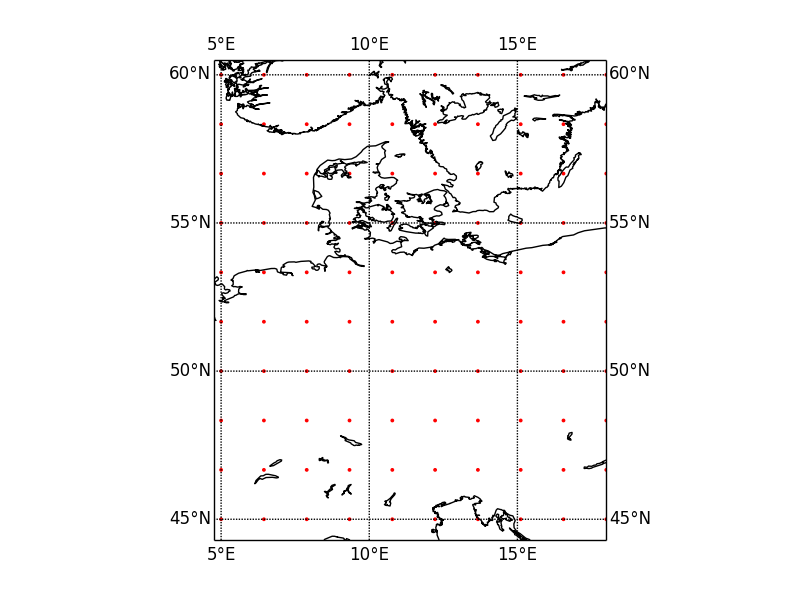
\includegraphics[scale=0.4]{/Users/student/seminar/bsp/bspscatter}\newpage 
   \subsubsection{Linienzüge zeichnen}
   Linienzüge lassen sich mit der Funktion \textsf{plot(x,y,**kw)} zeichnen. Diese Funktion zeichnet einen Linie von einem Punkt zum Nächsten. Dabei kann man \textsf{x,y} einfach als Felder übergeben. Hierbei ist zu beachten das davon ausgegangen wird das die Koordinaten Projektionskoordinaten sind.